\subsection{Layer 2 (Data Link)}
\subsection*{Aufgaben}
\begin{itemize}
	\item lokale Adressierung
	\item Fehlererkennung
	\item Zugang zum Medium herstellen
	\item Kommunikation mit Layer 3
\end{itemize}

\textbf{Geräte:} Netzwerkkarte, Switch, Bridge,... \\
\textbf{Standards:} Wifi (802.11), Ethernet (802.2, 802.3)
\subsection*{Topologie}
\begin{itemize}
	\item Sterntopologie
	\item Baumtopologie
	\item Punkt-zu-Punkt
\end{itemize}
\begin{figure}[H]
	\centering
	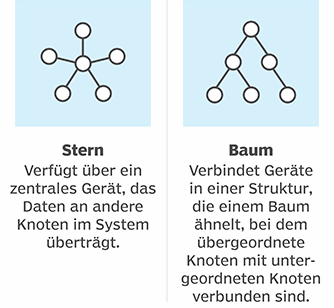
\includegraphics[width=0.6\linewidth]{figures/topologiearten.png}
	\caption{Baum- und Sterntopologie}
\end{figure}

\subsection*{Ethernet}
\begin{figure}[H]
	\centering
	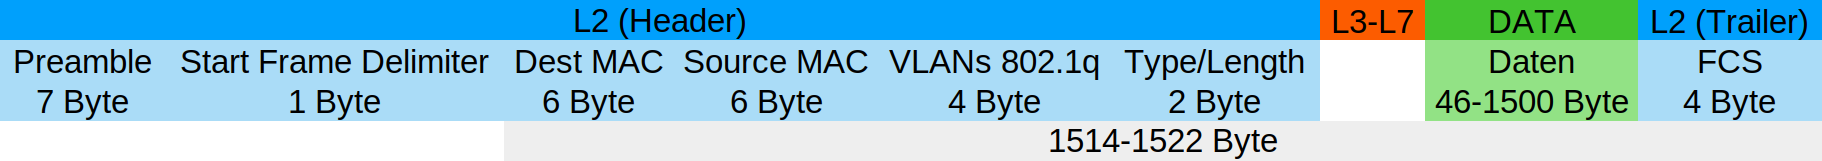
\includegraphics[width=1.0\linewidth]{figures/ethheader.png}
	\caption{Ethernet Frame}
\end{figure}

\subsection*{MAC-Adresse}
Die MAC-Adresse ist eine 48-Bit Zahl und wird in hexadecimal dargestellt.
\begin{tabbing}
	Bsp:\\
	Hersteller ~ \= für den Hersteller einzigartig \\
	DC F5 05 $\vert$\= 17 9A 69 \\
\end{tabbing}

Jede Netzwerkkarte besitzt eine weltweit einzigartige (theoretisch) MAC-Adresse.

\subsection*{Type}
Kodierung für Layer 3 \\
0x800 $\rightarrow$ IP \\
0x806 $\rightarrow$ ARP 

\subsection*{Fehlerkennung}
Frame Checksum (CRC) \\
Polynomdivision mit einem Polynom von Grad 32

\subsection*{Funktion eines Switches}
Der Switch baut mit der Source-MAC seine MAC-Tabelle auf. Dort steht zu jeder MAC-Adresse der passende Port. Falls die MAC-Adresse schon eingetragen ist, wird ein Timer aktualisiert. Sollte es noch keinen Eintrag geben wird er hinzugefügt und bleibt dort eine gewisse Zeit (5 Minuten) bevor er gelöscht wird. Der Switch vergleicht die Destination-MAC mit seiner MAC-Tabelle. Falls der Switch keinen Eintrag findet sendet er an alle Ports (Flooding, Unknown Unicast). Sonst sendet er an den Port, wo er den Frame bekommen hat. \\
Layer 2 Broadcast Adresse: FF:FF:FF:FF:FF:FF

\subsection*{L2, L3 Adressierung}
\begin{figure}[H]
	\centering
	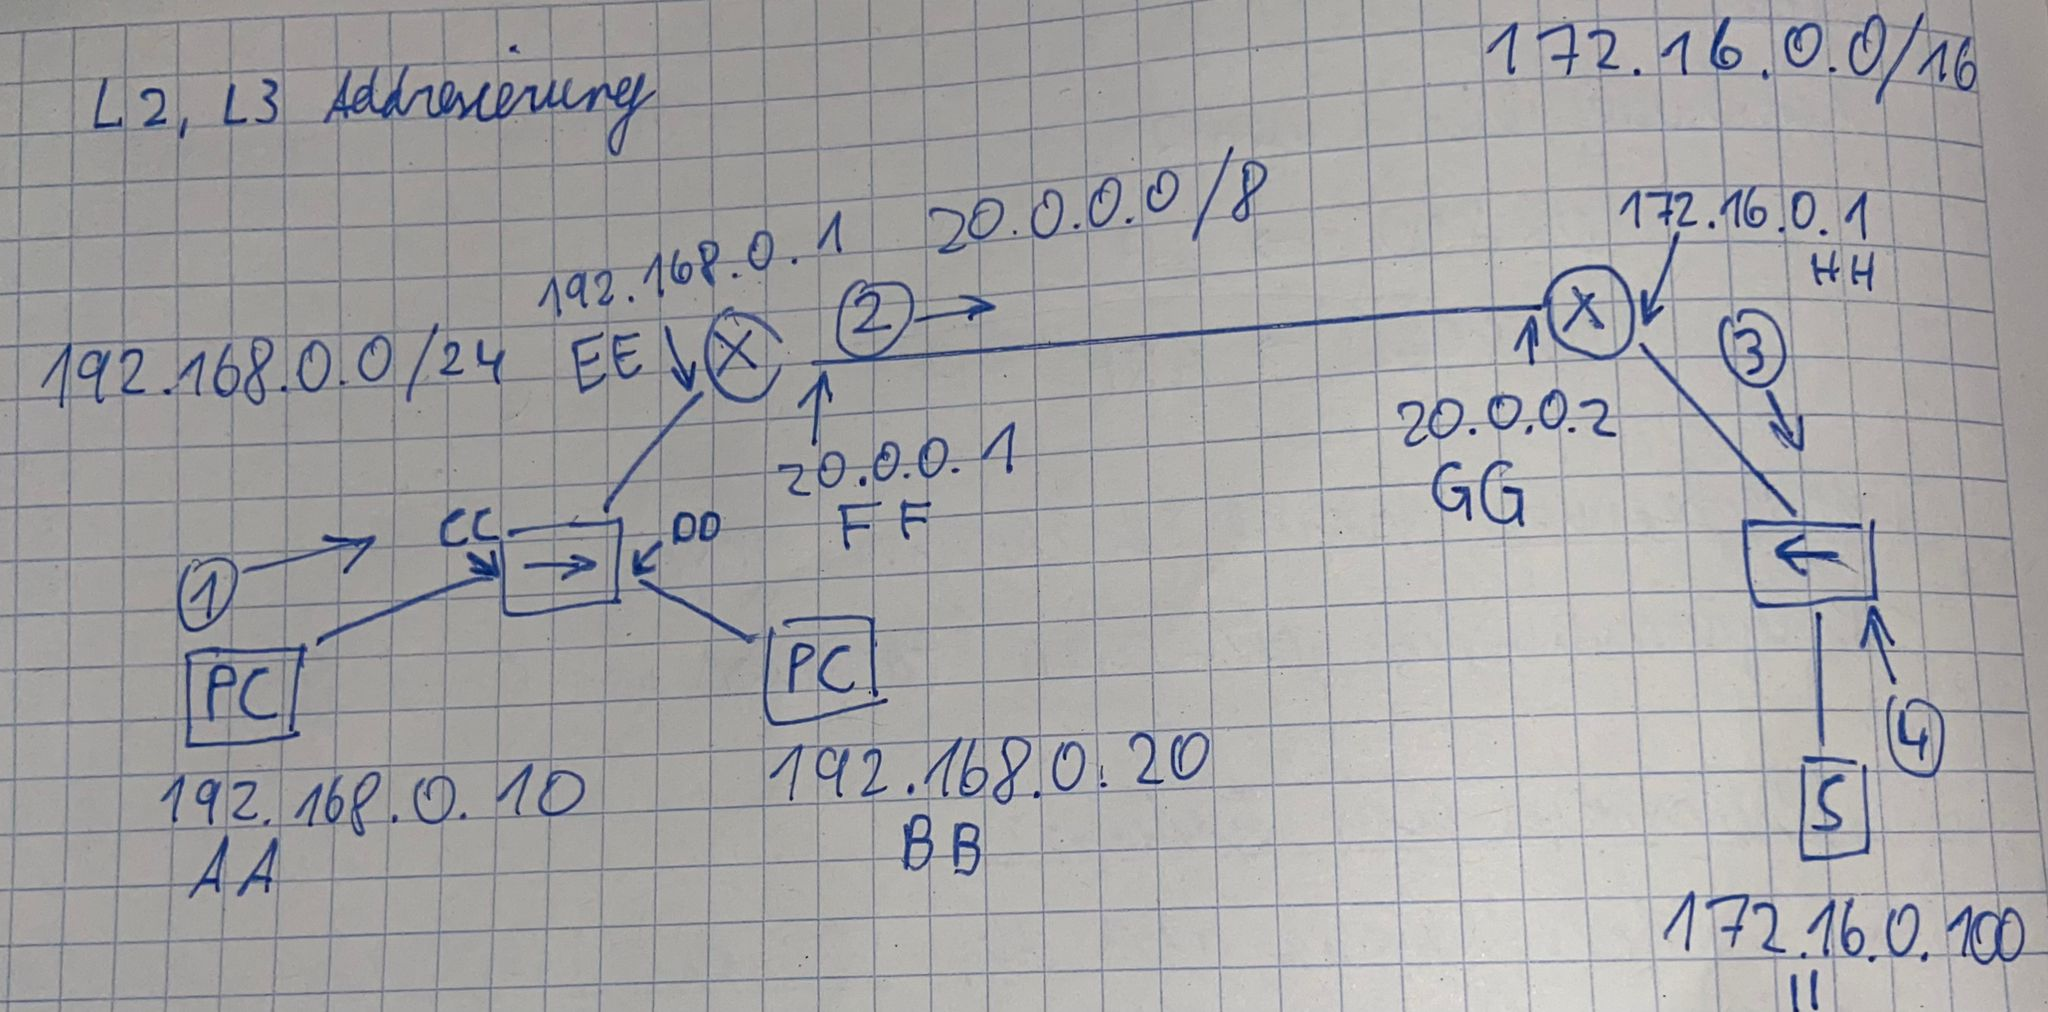
\includegraphics[width=1.0\linewidth]{figures/l2l3add.jpeg}
	\caption{Layer 2 \& 3 Adressierung}
\end{figure}

\begin{table}[H]
	\begin{tabular}{c|cccc}
		& Source MAC & Destination MAC & Source IP & Destination IP \\
		\hline
		1 & AA & EE & 192.168.0.10 & 172.16.0.100 \\
		2 & FF & GG & 192.168.0.10 & 172.16.0.100 \\
		3 & HH & II & 192.168.0.10 & 172.16.0.100 \\
		4 & II & HH & 172.16.0.100 & 192.168.0.10
	\end{tabular}
\end{table}

\subsection*{ARP (Address Resolution Protocol)}
Nutzt ein Host um zu einer gegebenen IP-Adresse die passende MAC-Adresse zu finden

\subsubsection*{ARP-Request (Broadcast)}
Source MAC: eigene MAC-Adresse \\
Destination MAC: FF-FF-FF-FF-FF-FF \\
Type: 0x806
Danach ARP-Header (IP, MAC, Protokoll)

\subsubsection*{ARP-Reply}
Unicast (auch als Broadcast möglich) \\
Source MAC: eigene MAC-Adresse (gesucht) \\
Destination MAC: MAC-Adresse (Anfrage) \\
Type: 0x806 \\
Danach ARP-Header

\subsubsection*{ARP-Cache}
Die Einträge werden im ARP-Cache gespeichert (ca 5 min) \\
IP MAC Time

\subsection*{ARP-Spoofing}
\begin{figure}[H]
	\centering
	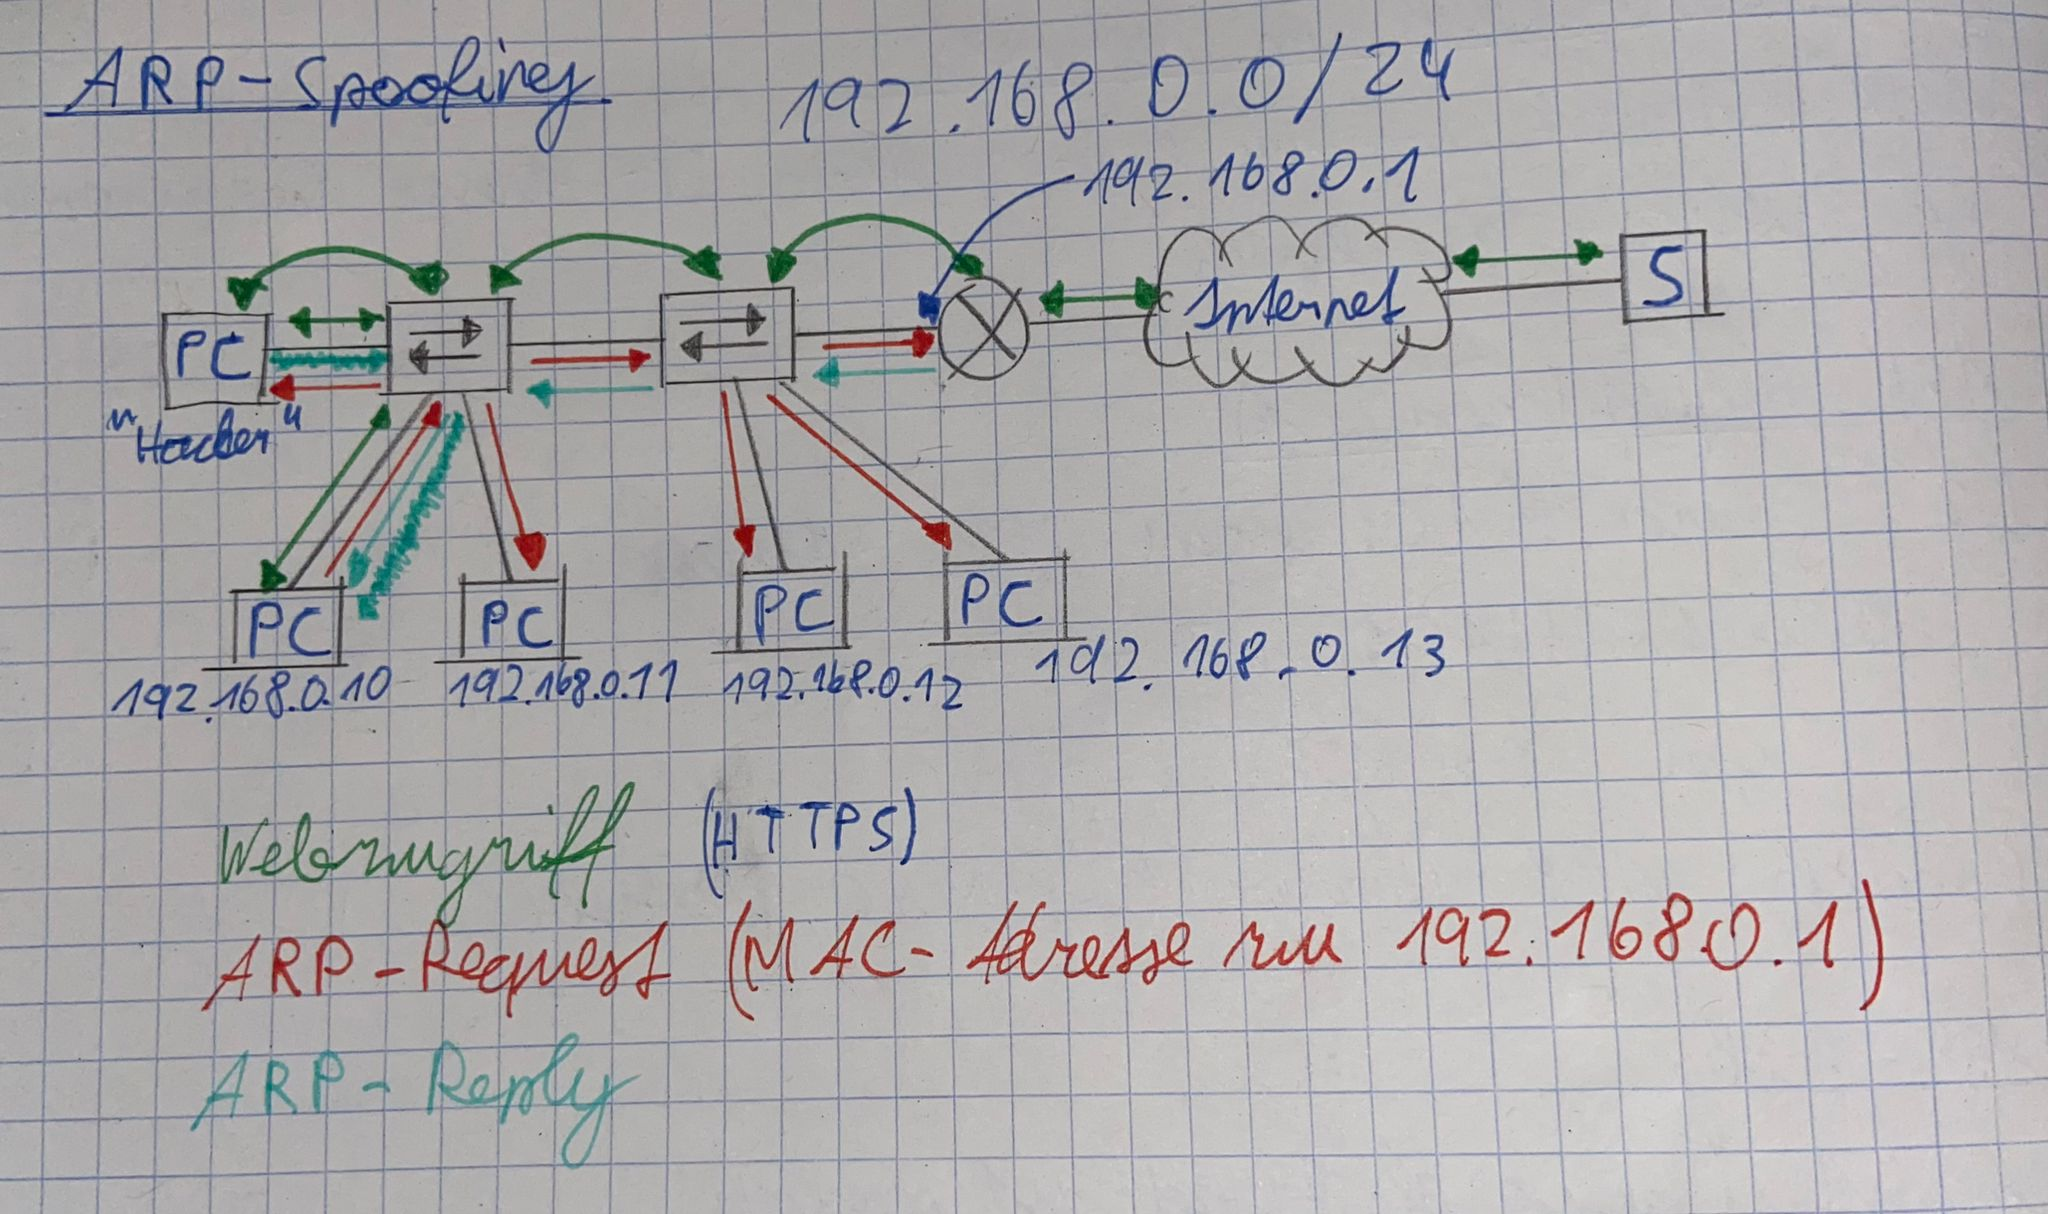
\includegraphics[width=1.0\linewidth]{figures/arpspoofing.jpeg}
	\caption{ARP-Spoofing}
\end{figure}





